\documentclass[14pt,a4paper,report]{report}
\usepackage[a4paper, mag=1000, left=2.5cm, right=1cm, top=2cm, bottom=2cm, headsep=0.7cm, footskip=1cm]{geometry}
\usepackage[utf8]{inputenc}
\usepackage[english,russian]{babel}
\usepackage{indentfirst}
\usepackage[dvipsnames]{xcolor}
\usepackage[colorlinks]{hyperref}
\usepackage{listings} 
\usepackage{fancyhdr}
\usepackage{caption}
\usepackage{amsmath}
\usepackage{latexsym}
\usepackage{graphicx}
\usepackage{amsmath}
\usepackage{booktabs}
\usepackage{array}
\hypersetup{
	colorlinks = true,
	linkcolor  = black
}

\usepackage{titlesec}
\titleformat{\chapter}
{\Large\bfseries} % format
{}                % label
{0pt}             % sep
{\huge}           % before-code


\DeclareCaptionFont{white}{\color{white}} 

% Listing description
\usepackage{listings} 
\DeclareCaptionFormat{listing}{\colorbox{gray}{\parbox{\textwidth}{#1#2#3}}}
\captionsetup[lstlisting]{format=listing,labelfont=white,textfont=white}
\lstset{ 
	% Listing settings
	inputencoding = utf8,			
	extendedchars = \true, 
	keepspaces = true, 			  	 % Поддержка кириллицы и пробелов в комментариях
	language = C++,            	 	 % Язык программирования (для подсветки)
	basicstyle = \small\sffamily, 	 % Размер и начертание шрифта для подсветки кода
	numbers = left,               	 % Где поставить нумерацию строк (слева\справа)
	numberstyle = \tiny,          	 % Размер шрифта для номеров строк
	stepnumber = 1,               	 % Размер шага между двумя номерами строк
	numbersep = 5pt,              	 % Как далеко отстоят номера строк от подсвечиваемого кода
	backgroundcolor = \color{white}, % Цвет фона подсветки - используем \usepackage{color}
	showspaces = false,           	 % Показывать или нет пробелы специальными отступами
	showstringspaces = false,    	 % Показывать или нет пробелы в строках
	showtabs = false,           	 % Показывать или нет табуляцию в строках
	frame = single,              	 % Рисовать рамку вокруг кода
	tabsize = 2,                  	 % Размер табуляции по умолчанию равен 2 пробелам
	captionpos = t,             	 % Позиция заголовка вверху [t] или внизу [b] 
	breaklines = true,           	 % Автоматически переносить строки (да\нет)
	breakatwhitespace = false,   	 % Переносить строки только если есть пробел
	escapeinside = {\%*}{*)}      	 % Если нужно добавить комментарии в коде
}

\begin{document}

\def\contentsname{Содержание}

% Titlepage
\begin{titlepage}
	\begin{center}
		\textsc{Санкт-Петербургский Политехнический 
			Университет Петра Великого\\[5mm]
			Кафедра компьютерных систем и программных технологий}
		
		\vfill
		
		\textbf{Отчёт по лабораторной работе №3\\[3mm]
			Курс: «Администрирование компьютерных сетей»\\[3mm]
			Тема: «Администрирование сетевых сервисов»\\[35mm]
			}
	\end{center}
	
	\hfill
	\begin{minipage}{.5\textwidth}
		Выполнил студент:\\[2mm] 
		Бояркин Никита Сергеевич\\
		Группа: 13541/3\\[5mm]
		
		Проверил:\\[2mm] 
		Малышев Игорь Алексеевич
	\end{minipage}
	\vfill
	\begin{center}
		Санкт-Петербург\\ \the\year\ г.
	\end{center}
\end{titlepage}

% Contents
\tableofcontents
\clearpage

\chapter{Лабораторная работа №3}

\section{Цель работы}

\begin{itemize}
	\item Изучение состава и функциональных возможностей сетевых сервисов операционных систем.
	\item Разработка и настройка сервисов локальной сети.
	\item Разработка и настройка сервисов демилитаризованной зоны.
	\item Разработка и настройка сервисов пограничной зоны.
\end{itemize}

\section{DHCP и удаленная загрузка}

В данной работе используются два DHCP сервера, на FreeBSD и на Ubuntu, для двух бездисковых клиентов из разных сетей. Также на Ubuntu будет установлен TFTP сервер для удаленной загрузки ОС.

\subsection{Структура сети}

\begin{figure}[h!]
	\centering
	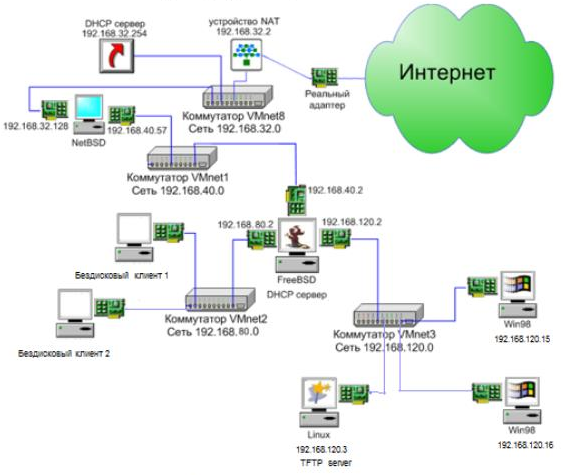
\includegraphics[scale = 0.95]{images/0_0.png}
	\caption{Модифицированная структура сети}
	\label{image:0}
\end{figure}

\clearpage

\subsection{Настройка DHCP на FreeBSD}

В первую очередь необходимо установить DHCP сервер из каталога /usr/ports/net/isc-dhcp44-server. После этого необходимо сконфигурировать DHCP сервер:

\begin{figure}[h!]
	\centering
	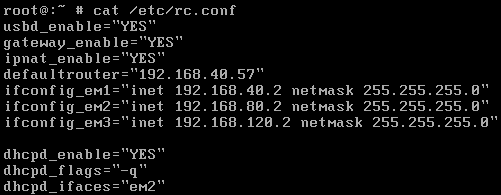
\includegraphics[scale = 1.1]{images/1_0.png}
	\caption{Конфигурация для DHCP сервера}
	\label{image:2}
\end{figure}

\begin{figure}[h!]
	\centering
	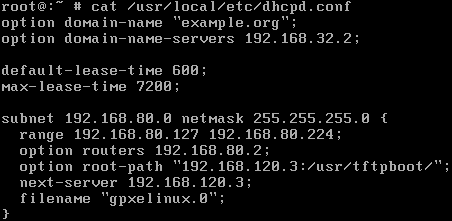
\includegraphics[scale = 1.1]{images/1_1.png}
	\caption{Конфигурация для DHCP сервера}
	\label{image:3}
\end{figure}

Запуск DHCP сервера:

\begin{figure}[h!]
	\centering
	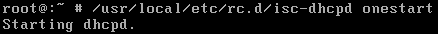
\includegraphics[scale = 1.1]{images/1_2.png}
	\caption{Запуск службы DHCP}
	\label{image:4}
\end{figure}

\subsection{Настройка DHCP на Ubuntu}

В первую очередь необходимо установить DHCP сервер командой:

\begin{lstlisting}
sudo apt-get install isc-dhcp-server
\end{lstlisting}

\clearpage

После этого необходимо сконфигурировать DHCP сервер:

\begin{figure}[h!]
	\centering
	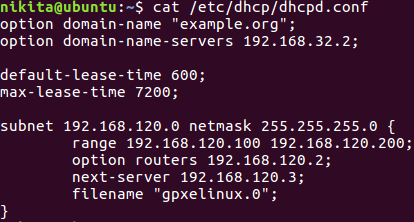
\includegraphics[scale = 0.87]{images/2_0.png}
	\caption{Конфигурация для DHCP сервера}
	\label{image:5}
\end{figure}

\begin{figure}[h!]
	\centering
	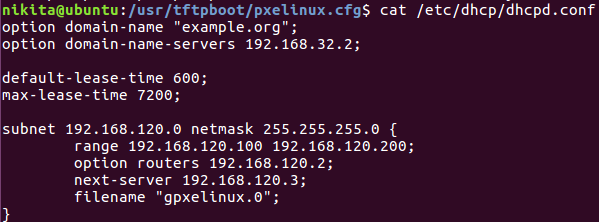
\includegraphics[scale = 0.87]{images/2_2.png}
	\caption{Конфигурация для DHCP сервера}
	\label{image:6}
\end{figure}

Запуск DHCP сервера:

\begin{figure}[h!]
	\centering
	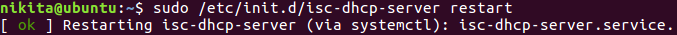
\includegraphics[scale = 1.0]{images/2_1.png}
	\caption{Запуск службы DHCP}
	\label{image:7}
\end{figure}

\subsection{Настройка TFTP на Ubuntu}

После установки TFTP необходимо создать каталог для удаленной загрузки:

\begin{figure}[h!]
	\centering
	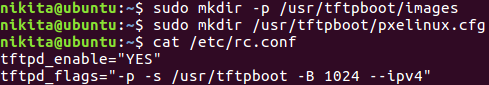
\includegraphics[scale = 1.1]{images/2_3.png}
	\caption{Создание каталога удаленной загрузки и настройка rc.conf}
	\label{image:8}
\end{figure}

После этого смонтируем образ Ubuntu в каталог удаленной загрузки:

\begin{figure}[h!]
	\centering
	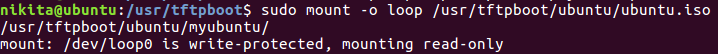
\includegraphics[scale = 0.8]{images/2_4.png}
	\caption{Монтирование образа в каталог удаленной загрузки}
	\label{image:9}
\end{figure}

\clearpage

Добавим общий доступ к данному каталогу:

\begin{figure}[h!]
	\centering
	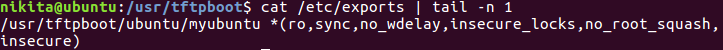
\includegraphics[scale = 0.85]{images/2_5.png}
	\caption{Внесение каталога удаленной загрузки в /etc/exports}
	\label{image:10}
\end{figure}

Зададим главный конфигурационный файл TFTP:

\begin{figure}[h!]
	\centering
	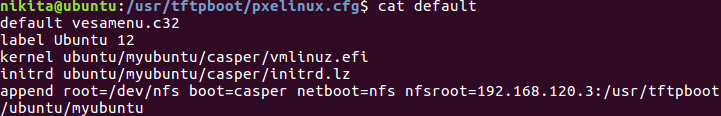
\includegraphics[scale = 0.85]{images/2_6.png}
	\caption{Конфигурационный файл удаленной загрузки}
	\label{image:11}
\end{figure}

\subsection{Тестирование}

В результате бездисковые клиенты могут автоматически подключаться к DHCP и устанавливать Ubuntu удаленно:

\begin{figure}[h!]
	\centering
	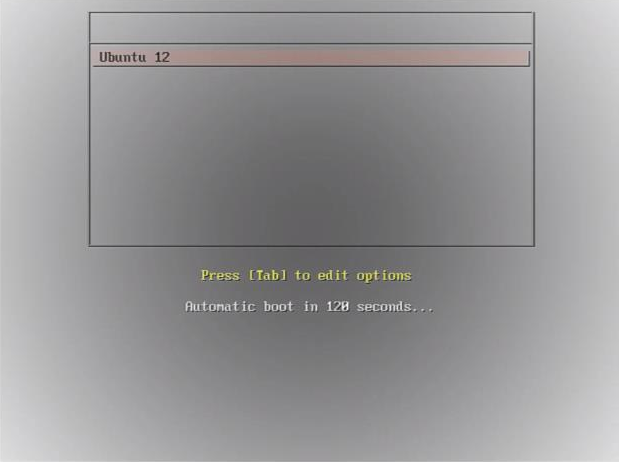
\includegraphics[scale = 0.85]{images/2_7.png}
	\caption{Окно загрузки Ubuntu на бездисковом клиенте}
	\label{image:12}
\end{figure}

\clearpage

\section{DNS сервисы}

Настроим кэширующий DNS сервер, а также связку из первичного и вторичного DNS серверов.

\subsection{Структура сети}

\begin{figure}[h!]
	\centering
	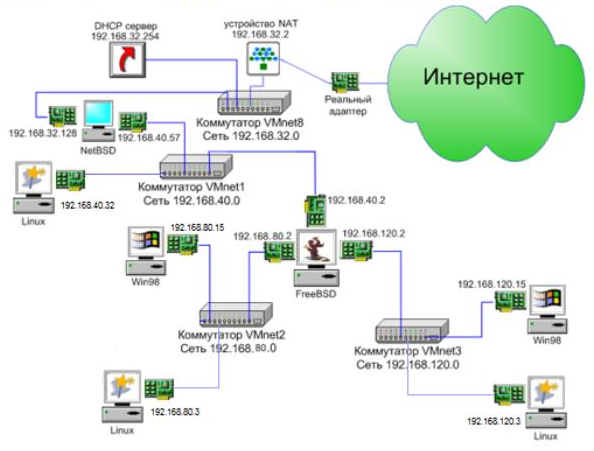
\includegraphics[scale = 0.9]{images/0_1.png}
	\caption{Модифицированная структура сети}
	\label{image:1}
\end{figure}

\subsection{Настройка кэширующего DNS сервера}

Настроим кэширующий DNS сервер на машине с адресом 192.168.40.32. Установим пакет bind9 для создания DNS сервера:

\begin{lstlisting}
sudo apt-get install bind9
\end{lstlisting}

Настроим DNS сервер:

\begin{figure}[h!]
	\centering
	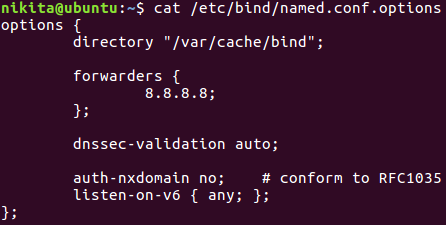
\includegraphics[scale = 1.0]{images/3_1.png}
	\caption{Настройка кэширующего DNS сервера}
	\label{image:13}
\end{figure}

Настроим клиент для данного сервера:

\begin{figure}[h!]
	\centering
	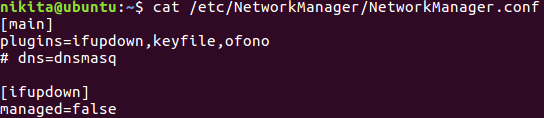
\includegraphics[scale = 1.1]{images/3_2.png}
	\caption{Настройка клиента для использования собственного DNS сервера}
	\label{image:14}
\end{figure}

\subsection{Тестирование}

Проверим работоспособность DNS сервера с помощью утилиты nslookup:

\begin{figure}[h!]
	\centering
	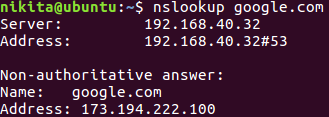
\includegraphics[scale = 1.1]{images/3_3.png}
	\caption{Проверка работы DNS сервера}
	\label{image:15}
\end{figure}

Проверим способность к кэшированию: замерим время запроса в первый раз и во второй раз:

\begin{figure}[h!]
	\centering
	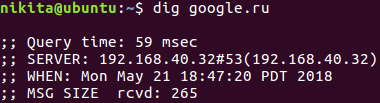
\includegraphics[scale = 1.1]{images/3_4.png}
	\caption{Первое обращение к DNS серверу}
	\label{image:16}
\end{figure}

\begin{figure}[h!]
	\centering
	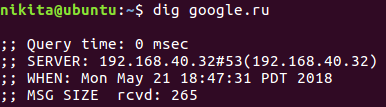
\includegraphics[scale = 1.1]{images/3_5.png}
	\caption{Второе обращение к DNS серверу}
	\label{image:17}
\end{figure}

Время второго запроса практически равно нулю, что означает, что кэширование работает.

\clearpage

\subsection{Настройка первичного DNS сервера}

Настроим первичный DNS сервер на машине с адресом 192.168.40.32:

\begin{figure}[h!]
	\centering
	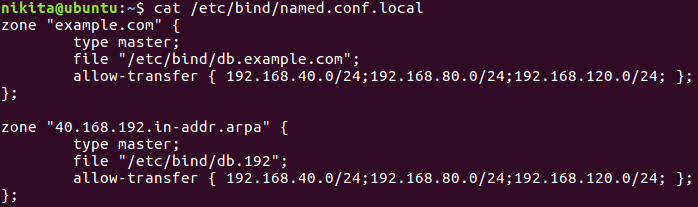
\includegraphics[scale = 0.9]{images/4_1.png}
	\caption{Конфигурация первичного DNS сервера}
	\label{image:18}
\end{figure}

\begin{figure}[h!]
	\centering
	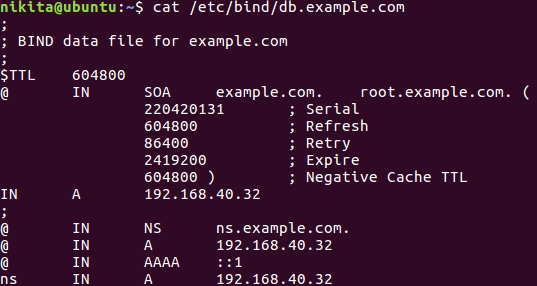
\includegraphics[scale = 0.9]{images/4_2.png}
	\caption{Конфигурация первичного DNS сервера}
	\label{image:19}
\end{figure}

\begin{figure}[h!]
	\centering
	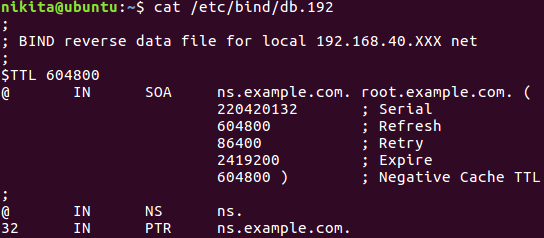
\includegraphics[scale = 0.9]{images/4_3.png}
	\caption{Конфигурация первичного DNS сервера}
	\label{image:20}
\end{figure}

\clearpage

\subsection{Настройка вторичного DNS сервера}

Настроим вторичный DNS сервер на машине с адресом 192.168.120.3.

\begin{figure}[h!]
	\centering
	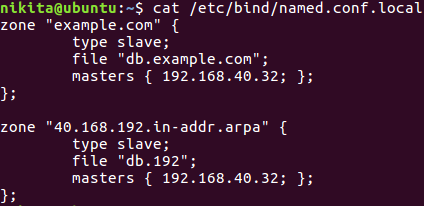
\includegraphics[scale = 0.9]{images/4_4.png}
	\caption{Конфигурация вторичного DNS сервера}
	\label{image:21}
\end{figure}

\subsection{Тестирование}

Проверим работу связки первичного и вторичного DNS серверов с помощью syslog:

\begin{figure}[h!]
	\centering
	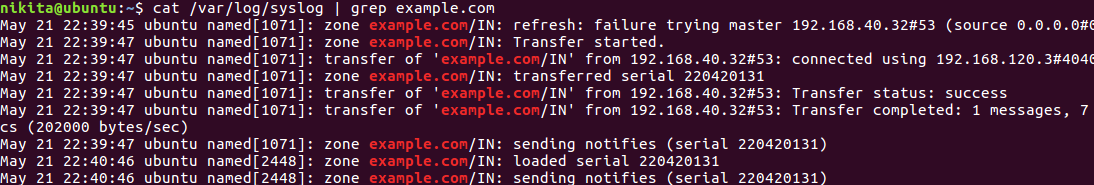
\includegraphics[scale = 0.6]{images/4_5.png}
	\caption{Результат работы связки первичного и вторичного DNS серверов}
	\label{image:22}
\end{figure}


\section{Вывод}

Сервера DHCP и удаленная загрузка значительно упрощают работу с сетью для пользователей, что делает эти технологии очень полезными в корпоративных сетях. Кроме того удаленная загрузка позволяет поддерживать одинаковую версию ПО для всех пользователей.

Кэширующий DNS сервер чрезвычайно эффективен при частом доступе к одинаковым ресурсам, как чаще всего и происходит при использовании интернет-ресурсов человеком.




\end{document}